\documentclass[xcolor=dvipsnames,mathserif,9pt]{beamer} %handout
%\usefonttheme{serif}%{structurebold}%{structuresmallcapsserif}%{serif}

\usepackage{graphicx}
\usepackage{amsmath}
\usepackage{amssymb}
\usepackage[font=footnotesize]{caption} % set the captain font size to 8 (i.e. footnotesize)
\usepackage{subfig} % uses subfloats within a single float MUST after the package {caption}!!
\usepackage{natbib}
%\usepackage{cite} % sort the reference in the article by number or alphabatic
\usepackage{color}
\usepackage{algorithm} % options: boxed [section]
\usepackage{algpseudocode} % for algorithm
%\usepackage{enumerate}
\usepackage{enumitem} % directly use itemize, easily specify indent and everything
\setlist[itemize]{leftmargin=*,label=$\bullet$}%leftmargin=*,itemsep=0pt} %topsep=5pt
\setlist[enumerate]{label={\arabic*)}}
\usepackage{hyperref}
\usepackage{wrapfig}
\usepackage{textpos}
\usepackage{bibentry} % for publication list
\makeatletter\let\saved@bibitem\@bibitem\makeatother % make hyperref and bibentry compatible!!!
\nobibliography*
\usepackage{fancybox}% shadow for image
%\usepackage{empheq} % emphasize equations
\usepackage{bm}
\usepackage{arydshln} % for dashline in table or matrix
\linespread{1.3}
\usepackage{multimedia}

\usepackage{setspace} \setstretch{1.2}

\usepackage{framed}
\colorlet{shadecolor}{black!5}
% for box, page breakable, very good!!
\usepackage[framemethod=TikZ]{mdframed}%
\mdfdefinestyle{myFrame}{%
    linecolor=gray!15!white,%gray
    outerlinewidth=0.1pt,
    roundcorner=3pt,
    skipabove=15pt, % the space before the entire box
    skipbelow=15pt, % the space after the entire box. Please see the figure 2 in the manual, very clear!
    innertopmargin=10pt,%\baselineskip,
    innerbottommargin=10pt,%\baselineskip,
    %innerrightmargin=10pt,
    %innerleftmargin=10pt,
    splittopskip=\baselineskip,
    splitbottomskip=\baselineskip,
    backgroundcolor=gray!10!white,
    frametitlerule=true,
    frametitlebackgroundcolor=gray!20!white,
    frametitleaboveskip=5pt,
    frametitlebelowskip=5pt,
}
\mdfdefinestyle{myAlgo}{%
    linecolor=gray!100!white,%gray
    outerlinewidth=0.1pt,
    roundcorner=3pt,
    skipabove=15pt, % the space before the entire box
    skipbelow=15pt, % the space after the entire box. Please see the figure 2 in the manual, very clear!
    innertopmargin=10pt,%\baselineskip,
    innerbottommargin=10pt,%\baselineskip,
    %innerrightmargin=10pt,
    %innerleftmargin=10pt,
    splittopskip=\baselineskip,
    splitbottomskip=\baselineskip,
    backgroundcolor=gray!0!white,
    frametitlerule=true,
    frametitlebackgroundcolor=gray!20!white,
    frametitleaboveskip=5pt,
    frametitlebelowskip=5pt,
}


\usepackage{tikz}
\usetikzlibrary{calc} % for calculation functions in Tikz let, in commands in Tikz
\usetikzlibrary{shapes} % for block diagram
\usetikzlibrary{chains}
\usetikzlibrary{fit}
\usetikzlibrary{arrows}
\usetikzlibrary{decorations.text} % text along path

\newcommand{\blue}[1]{\textcolor{blue}{#1}}
\definecolor{myred}{RGB}{200,0,0}
\newcommand{\red}[1]{\textcolor{myred}{#1}} %magenta purple
\newcommand{\I}{\mathcal{I}}
\newcommand{\tr}{\mathrm{tr}}
\newcommand{\Null}{\mathrm{Null}}
\newcommand{\Range}{\mathrm{Range}}
\newcommand{\one}{\mathbf{1}}
\newcommand{\rank}{\mathrm{rank}}
\newcommand{\myspan}{\mathrm{span}}
\newcommand{\mydiag}{\mathrm{diag}}
\newcommand{\D}{\mathrm{d}}
\renewcommand{\d}{\mathrm{d}}
\newcommand{\blkdiag}{\mathrm{blkdiag}}
\newcommand{\sgn}{\mathrm{sgn}}
\newcommand{\T}{\mathrm{T}}
\newcommand{\myqed}{\hfill$\blacksquare$}
\newcommand{\ep}{\varepsilon}
\newcommand{\sig}{\mathrm{sig}_a}
%\newcommand{\sigep_}[1]{\sig(\ep_{#1})}
\newcommand{\R}{\mathbb{R}}
\newcommand{\A}{\mathcal{A}}
\newcommand{\G}{\mathcal{G}}
\newcommand{\E}{\mathbb{E}}
\newcommand{\X}{\mathcal{X}}
\newcommand{\V}{\mathcal{V}}
\newcommand{\N}{\mathcal{N}}
\newcommand{\M}{\mathcal{M}}
\renewcommand{\H}{\mathcal{H}}
\renewcommand{\L}{\mathcal{B}}
\renewcommand{\S}{\mathcal{S}}
\newcommand{\xe}{x_{\text{e}}}
%\newcommand{\Null}[1]{\mathrm{Null}\left(#1\right)}
\newcommand{\sk}[1]{\left[#1\right]_\times} % skew symmetric operator
\newcommand{\dia}[1]{\mathrm{diag}\left(#1\right)} % block diagnal matrix
%\renewcommand{\span}[1]{\mathrm{span}\left\{#1\right\}} % ERROR when redefine \span
\newcommand{\Var}{\mathrm{Var}}
\newcommand{\var}{\mathrm{var}}


\graphicspath{{figures/}}

% for tikz, theorem, lemma ... environments have already been declared. You don't need to declare, or you need to use other names than theorem or lemma, such as my_theorem.
%\newtheorem{my_theorem}{Theorem}
%\newtheorem{my_lemma}{Lemma}
\newtheorem{assumption}{Assumption} % necessary for beamer
%\newtheorem{my_remark}{Remark}
\newtheorem{proposition}{Proposition} % necessary for beamer
%\newtheorem{my_corollary}{Corollary}
%\newtheorem{my_example}{Example}
%\newtheorem{my_definition}{Definition}
%\newtheorem{my_problem}{Problem}

%##################################################
\newcommand{\pagetitle}[1]{\textbf{\textcolor{BlueViolet}{$\circ$ #1}}} %!!!
\newcommand{\pagehighlight}[1]{\textbf{\textcolor{Brown}{#1}}} %!!!
\newcommand{\mypause}{\pause} % this is useful for slide show. if you don't want pause any more, just set it as blank
%\newcommand{\mybullet}{\textcolor{BlueViolet}{$\blacksquare$} }%{$\rhd$ }
%\newcommand{\myhighsign}{$\star$ }% the sign to highlight a sentence

%##################################################
% To highlight equation. Example: \begin{align*} \boxed{xxx} \end{align*}
% does not support multiline equations
% put color to \boxed math command
\newcommand*{\boxcolor}{gray}
\makeatletter
\renewcommand{\boxed}[1]{\textcolor{\boxcolor}{%
%\tikz[baseline={([yshift=-1ex]current bounding box.center)}] \node [rectangle, minimum width=1ex,rounded corners,draw] {\normalcolor\m@th$\displaystyle#1$};}}
\tikz[baseline={([yshift=-1ex]current bounding box.center)}] \node [rectangle, minimum width=2ex,rounded corners,draw] {\normalcolor\m@th$\displaystyle#1$};}}
\makeatother

%##################################################
% set my own theme
\def\structureHeight{9mm}
\usetheme[height=\structureHeight]{Rochester}
\usecolortheme[RGB={0,0,128}]{structure}
\setbeamertemplate{items}[circle]%rectangle, triangle,circle
\setbeamertemplate{blocks}[rounded][shadow=true]
\setbeamertemplate{navigation symbols}{}
%\addtobeamertemplate{frametitle}{} % specify the logo
%{
%    \begin{textblock*}{100mm}(.87\textwidth,-\structureHeight)
%        \includegraphics[height=6.6mm,width=3cm,keepaspectratio]{../common_figures_private/westlake_logo.png} % add logo
%    \end{textblock*}
%}
\addtobeamertemplate{frametitle}{\vskip4pt}{} % specify
%\setbeamerfont{frametitle}{size=\large}
\definecolor{mylightgray}{RGB}{240 240 240}
\definecolor{mykhaki}{RGB}{240 230 140}% khaki color
\definecolor{mylightYellow}{RGB}{255,255,224} % light yellow
%\setbeamercolor{beamercolor1}{bg=mylightgray, fg=black}
%\setbeamercolor{beamercolor2}{bg=mylightYellow,fg=black}%{bg=yellow!90!white, fg=black}
% background and foreground color
\setbeamercolor{background canvas}{bg=black!0!white} % background color of every slide! My previous value was black!10!white for my lecture videos!
\setbeamercolor{normal text}{bg=black!10!white} % background color for e.g. theorem environment. When canvas is 10, here it can be 20; the bg for normal text changes the color of hidden text when you use overlay

\setbeamercolor{block title}{bg=mykhaki,fg=black}
\defbeamertemplate{footline}{zsy_frameNumber}
{%
  \hspace{5pt}  \emph{Shiyu Zhao}
  \hspace*{\fill}%
  \usebeamercolor[fg]{page number in head/foot}%
  \insertframenumber\,/\,\inserttotalframenumber \vspace{0pt} \hspace{5pt}
  \vskip5pt
}
\setbeamertemplate{footline}[zsy_frameNumber]
%##################################################
\setbeamercovered{transparent=0} % a good value for transparent text is 20
% when using the overlay commands like \onslide or \uncover, the text will NOT be invisible, instead it will be like transparent
%\pause will also have the transparent effect: command \pause is easy to use: to make it invisible, change the value to zero.



\usepackage{multimedia}

%\newcommand{\blue}[1]{\textcolor{blue}{#1}}
%\newcommand{\red}[1]{\textcolor{red}{#1}}
%\newcommand{\I}{\mathcal{I}}
\begin{document}

%%%%%%%%%%%%%%%%%%%%%%%%%%%%%%%%%%%%%%%%%%%%%%%%%%%%%%%%%%%%%%%%%%%%%%%%%%%%%%%%%
% define the author, date etc. information
%\subtitle{Mathematical and Biological Foundation for Reinforcement Learning}
\title{Lecture 2: State Value and Bellman Equation}

\author{Shiyu Zhao
\newline
\newline {\small Department of Artificial Intelligence}
\newline {\small Westlake University}
}
%\logo{\includegraphics[width=1cm,height=1cm,keepaspectratio]{NUSLogo.png}~}
%\date{\today}
\date{}
\subject{}


%%%%%%%%%%%%%%%%%%%%%%%%%%%%%%%%%%%%%%%%%%%%%%%%%%%%%%%%%%%%%%%%%%%%%%%%%%%%%%%%%

{
\setbeamertemplate{footline}{} % remove the frame number of the title page
\begin{frame}
    %\frametitle{Lecture: Networked Dynamic Systems}
    \addtocounter{framenumber}{-1} % discounter the title page, otherwise the frame number starts from 2 instead of 1
    \titlepage % this only gives the author etc. information
\end{frame}
}


\begin{frame}
\frametitle{Outline}
\begin{figure}[h]
  \centering
\includegraphics[width=0.8\linewidth]{Figure_chapterRelationship.pdf}
\end{figure}
\end{frame}

\begin{frame}
\frametitle{Introduction}

\begin{itemize}
\item This lecture introduces temporal-difference (TD) learning, which is one of the most well-known methods in reinforcement learning (RL).
\item Monte Carlo (MC) learning is the first model-free method. TD learning is the second model-free method. TD has some advantages compared to MC.
\item We will see how the stochastic approximation methods studied in the last lecture are useful.
\end{itemize}

\end{frame}
%---------------------
\begin{frame}
\frametitle{Outline}
\tableofcontents
\end{frame}
\AtBeginSection[]% put it to the start of each section
{
  \begin{frame}
    \frametitle{Outline}
    \tableofcontents[currentsection]
  \end{frame}
}
%--------------------------------------
\AtBeginSection[]% put it to the start of each section
{
  \begin{frame}
    \frametitle{Outline}
    \tableofcontents[currentsection]
  \end{frame}
}
\section{Motivating examples}
%---------------------
\begin{frame}
\frametitle{Motivating example: stochastic algorithms}

We next consider some stochastic problems and show how to use the \blue{RM algorithm} to solve them.

\pause
\textbf{First, \blue{revisit} the mean estimation problem:} calculate
\begin{align*}
w=\E[X]
\end{align*}
based on some iid samples $\{x\}$ of $X$. We studied it in the last lecture.
\begin{itemize}
\pause
\item
By writing $g(w)=w-\E[X]$, we can reformulate the problem to a root-finding problem
$$g(w)=0$$

\pause
\item
Since we can only obtain samples $\{x\}$ of $X$, the noisy observation is
$$\tilde{g}(w,\eta)=w-x=(w-\E[X])+(\E[X]-x)\doteq g(w)+\eta$$

\pause
\item
According to the last lecture, we know the RM algorithm for solving $g(w)=0$ is
\vspace{-5pt}
\begin{align*}
\blue{w_{k+1}=w_k-\alpha_k\tilde{g}(w_k,\eta_k)=w_k-\alpha_k(w_k-x_k)}
\end{align*}
%$w_k$ converges to $\E[X]$ with probability 1 if $\sum_{k=1}^\infty \alpha_k=\infty$ and $\sum_{k=1}^\infty \alpha_k^2<\infty$.
\end{itemize}

\end{frame}
%---------------------
\begin{frame}
\frametitle{Motivating example: stochastic algorithms}

\textbf{Second, consider a little more complex problem.} That is to estimate the mean of a function $v(X)$,
\begin{align*}
w=\E[v(X)],
\end{align*}
based on some iid random samples $\{x\}$ of $X$.

\begin{itemize}
\pause
\item To solve this problem, we define
\begin{align*}
g(w)&=w-\E[v(X)]\\
\tilde{g}(w,\eta)&=w-v(x)=(w\red{-\E[v(X)]})+(\red{\E[v(X)]}-v(x))\doteq g(w)+\eta.
\end{align*}

\pause
\item
Then, the problem becomes a root-finding problem: $g(w)=0$. The corresponding RM algorithm is
\begin{align*}
\blue{w_{k+1}=w_k-\alpha_k\tilde{g}(w_k,\eta_k)
=w_k-\alpha_k[w_k-v(x_k)]}
\end{align*}

\end{itemize}

\end{frame}
%---------------------
\begin{frame}
\frametitle{Motivating example: stochastic algorithms}

\textbf{Third, consider an even more complex problem:} calculate
\begin{align*}%\label{eq_TDMeanEstDemoEq}
w=\E[R+\gamma v(X)],
\end{align*}
where $R,X$ are random variables, $\gamma$ is a constant, and $v(\cdot)$ is a function.

\begin{itemize}
\pause
\item Suppose we can obtain samples $\{x\}$ and $\{r\}$ of $X$ and $R$.
We define
\begin{align*}
g(w)&=w-\E[R+\gamma v(X)],\\
\tilde{g}(w,\eta)&=w-[r+\gamma v(x)]\\
&=(w\red{-\E[R+\gamma v(X)]})+(\red{\E[R+\gamma v(X)]}-[r+\gamma v(x)])\\
&\doteq g(w)+\eta.
\end{align*}

\pause
\item
Then, the problem becomes a root-finding problem: $g(w)=0$. The corresponding RM algorithm is
\begin{align*}
\blue{w_{k+1}=w_k-\alpha_k\tilde{g}(w_k,\eta_k)
=w_k-\alpha_k[w_k-(r_k+\gamma v(x_k))]}
\end{align*}
This algorithm looks like TD algorithms as shown later.
\end{itemize}

\end{frame}
%---------------------
\begin{frame}
\frametitle{Motivating example: stochastic algorithms}

Quick summary:
\begin{itemize}
\item The above three examples become more and more complex.
\item They can all be solved by the RM algorithm.
\item We will see that the TD algorithms have similar expressions.
\end{itemize}
\end{frame}
%--------------------------------------
\AtBeginSection[]% put it to the start of each section
{
  \begin{frame}
    \frametitle{Outline}
    \tableofcontents[currentsection]
  \end{frame}
}
\section{TD learning of state values}
%%---------------------
%\begin{frame}
%\frametitle{TD learning of state values}
%
%Note that
%\begin{itemize}
%\item TD learning often refers to \blue{a broad class of RL algorithms.}
%\item TD learning also refers to \blue{a specific algorithm for estimating state values} as introduced below.
%\end{itemize}
%\end{frame}
%---------------------
\begin{frame}
\frametitle{TD learning of state values -- Algorithm description}

Problem statement:
\begin{itemize}
\item Given policy $\pi$, the aim is to estimate the state values $\{v_\pi(s)\}_{s\in\S}$ under $\pi$.
\item Experience samples: \blue{$(s_0,r_1,s_1,\dots,s_t,r_{t+1},s_{t+1},\dots)$} or \blue{$\{(s_t,r_{t+1},s_{t+1})\}_{t}$} generated by $\pi$.
\end{itemize}
\pause
Important notations:
\begin{gather*}
v(s) \longrightarrow v_\pi(s)\\
\visible<3->{
\Downarrow\\
v(s_{\red{t}}) \longrightarrow v_\pi(s_{\red{t}})\\}
\visible<4->{\Downarrow\\
v_{\red{t}}(s_{\red{t}}) \longrightarrow v_\pi(s_{\red{t}})}
\end{gather*}

\end{frame}
%---------------------
\begin{frame}
\frametitle{TD learning of state values -- Algorithm description}

\textbf{The TD learning algorithm is}
\red{
\begin{align}
v_{t+1}(s_t)&=v_t(s_t)-\alpha_t(s_t)\Big[v_t(s_t)-[r_{t+1}+\gamma v_t(s_{t+1})]\Big],\label{eq_TDAlgoStateValue}\\
v_{t+1}(s)&=v_{t}(s),\quad \forall s\ne s_t,\label{eq_TDAlgoStateValue2}
\end{align}}
where $t=0,1,2,\dots$.

\vspace{10pt}
Here, $v_t(s_t)$ is the estimated state value of $v_\pi(s_t)$; $\alpha_t(s_t)$ is the learning rate of $s_t$ at time $t$.
\begin{itemize}
\item At time $t$, only the value of the visited state $s_t$ is updated whereas the values of the unvisited states $s\ne s_t$ remain unchanged.
\item The update in \eqref{eq_TDAlgoStateValue2} will be omitted when the context is clear.
\end{itemize}
\end{frame}
%---------------------
\begin{frame}
\frametitle{TD learning of state values -- Algorithm properties}
The TD algorithm can be annotated as
\red{
\begin{align}\label{eq_TDAlgoStateValueAnnotated}
\underbrace{v_{t+1}(s_t)}_{\text{new estimate}}&=\underbrace{v_t(s_t)}_{\text{current estimate}}-\alpha_t(s_t)\big[\overbrace{v_t(s_t)-[\underbrace{r_{t+1}+\gamma v_t(s_{t+1})}_{\text{TD target }\bar{v}_t}]}^{\text{TD error $\delta_t$}}\big],
\end{align}}

\pause
Here,
$$\bar{v}_t\doteq r_{t+1}+\gamma v_t(s_{t+1})$$
is called the \blue{TD target}.
\pause
$$\delta_t\doteq v_t(s_t)-[r_{t+1}+\gamma v_t(s_{t+1})]=v_t(s_t)-\bar{v}_t$$
is called the \blue{TD error}.

\vspace{10pt}
\pause
Observation: The new estimate $v_{t+1}(s_t)$ is a combination of the current estimate $v_t(s_t)$ and the TD error.

\end{frame}
%---------------------
\begin{frame}
\frametitle{TD learning of state values -- Algorithm properties}

\textbf{First, why is $\bar{v}_t$ called the TD target?}

\pause
\blue{That is because the algorithm drives $v(s_t)$ towards $\bar{v}_t$.}

\pause
To see that,
\begin{align*}
&v_{t+1}(s_t)=v_t(s_t)-\alpha_t(s_t)\big[v_t(s_t)-\bar{v}_t\big]\\
\visible<4->{
\Longrightarrow \quad
&v_{t+1}(s_t)\blue{-\bar{v}_t}=v_t(s_t)\blue{-\bar{v}_t}-\alpha_t(s_t)\big[v_t(s_t)-\bar{v}_t\big]}\\
\visible<5->{\Longrightarrow \quad
&v_{t+1}(s_t)\blue{-\bar{v}_t}=[1-\alpha_t(s_t)][v_t(s_t)\blue{-\bar{v}_t}]}\\
\visible<6->{\Longrightarrow \quad
&|v_{t+1}(s_t)\blue{-\bar{v}_t}|=|1-\alpha_t(s_t)||v_t(s_t)\blue{-\bar{v}_t}|}
\end{align*}
\visible<7->{Since $\alpha_t(s_t)$ is a small positive number, we have
$$0<1-\alpha_t(s_t)<1$$}
\visible<8->{
Therefore,
\begin{align*}
|v_{t+1}(s_t)\blue{-\bar{v}_t}|\le|v_t(s_t)\blue{-\bar{v}_t}|
\end{align*}
which means $v(s_t)$ is driven towards $\bar{v}_t$!}
\end{frame}
%---------------------
\begin{frame}
\frametitle{TD learning of state values -- Algorithm properties}

\textbf{Second, what is the interpretation of the TD error?}
$$\delta_t=v_t(s_t)-[r_{t+1}+\gamma v_t(s_{t+1})]$$
\begin{itemize}
\pause
\item It reflects the \blue{difference} between \red{two time steps}.
\pause
\item It reflects the \blue{difference} between \red{$v_t$ and $v_{\pi}$}.
\pause
To see that, denote
$$\delta_{\pi,t}\doteq v_\pi(s_t)-[r_{t+1}+\gamma v_\pi(s_{t+1})]$$
\pause
Note that
\begin{align*}
&\E[\delta_{\pi,t}|S_t=s_t]=v_\pi(s_t)-\E\big[R_{t+1}+\gamma v_\pi(S_{t+1})|S_t=s_t\big]=0.
\end{align*}

\pause
\begin{itemize}
\item[-] \blue{If $v_t=v_\pi$, then $\delta_t$ should be zero (in the expectation sense).}
\item[-] Hence, if $\delta_t$ is not zero, then $v_t$ is not equal to $v_\pi$.
\end{itemize}
\pause
\item The TD error can be interpreted as \blue{innovation}, which means new information obtained from the experience $(s_t,r_{t+1},s_{t+1})$.
\end{itemize}
\end{frame}
%---------------------
\begin{frame}
\frametitle{TD learning of state values -- Algorithm properties}

Other properties:
\begin{itemize}
\item The TD algorithm in \eqref{eq_TDAlgoStateValueAnnotated} \blue{only estimates the state value of a given policy}.
\begin{itemize}
\item \emph{It does not estimate the action values.}
\item \emph{It does not search for optimal policies.}
\end{itemize}
\item This algorithm will be extended to estimate action values and then search for optimal policies later in this lecture.
\item The TD algorithm in \eqref{eq_TDAlgoStateValueAnnotated} is fundamental for understanding more complex TD algorithms.
\end{itemize}
\end{frame}
%---------------------
\begin{frame}
\frametitle{TD learning of state values -- The idea of the algorithm}

\textbf{Q: What does this TD algorithm do mathematically?}

\blue{A: It is a \red{model-free} algorithm for solving the Bellman equation of a given policy $\pi$.}
\begin{itemize}
\item Chapter 2 has introduced the \red{model-based} algorithm for solving the Bellman equation: closed-form solution + iterative algorithm.
\end{itemize}
\end{frame}
%---------------------
\begin{frame}
\frametitle{TD learning of state values -- The idea of the algorithm}

\textbf{First, a new expression of the Bellman equation.}

\pause
The definition of state value of $\pi$ is
\begin{align}\label{eq_TDDefOfStateValue}
v_\pi(s)=\E\big[R+\gamma G|S=s\big], \quad s\in\S
\end{align}
where $G$ is discounted return.
\pause
Since
\begin{align*}
\E[G|S=s]=\sum_{a}\pi(a|s)\sum_{s'} p(s'|s,a)\blue{v_\pi(s')}=\E[\blue{v_\pi(S')}|S=s],
\end{align*}
where $S'$ is the next state,
\pause
we can rewrite \eqref{eq_TDDefOfStateValue} as
\begin{align}\label{eq_TDBellmanEquationExpectationForm}
\blue{v_\pi(s)=\E\big[R+\gamma v_\pi(S')|S=s\big],\quad s\in\S.}
\end{align}
\pause
Equation~\eqref{eq_TDBellmanEquationExpectationForm} is another expression of the Bellman equation. It is sometimes called the \red{Bellman expectation equation}, an important tool to design and analyze TD algorithms.
\end{frame}
%---------------------
\begin{frame}
\frametitle{TD learning of state values -- The idea of the algorithm}

\textbf{Second, solve the Bellman equation in \eqref{eq_TDBellmanEquationExpectationForm} using the RM algorithm.}

In particular, by defining
\begin{align*}
g(v(s))=v(s)-\E\big[R+\gamma v_\pi(S')|s\big],
\end{align*}
we can rewrite \eqref{eq_TDBellmanEquationExpectationForm} as
$$g(v(s))=0.$$
\pause
Since we can only obtain the samples $r$ and $s'$ of $R$ and $S'$, the noisy observation we have is
{\small
\begin{align*}
\tilde{g}(v(s))
&=v(s)-\big[r+\gamma v_\pi(s')\big]\\
&=\underbrace{\Big(v(s)\blue{-\E\big[R+\gamma v_\pi(S')|s\big]}\Big)}_{g(v(s))}
+\underbrace{\Big(\blue{\E\big[R+\gamma v_\pi(S')|s\big]}-\big[r+\gamma v_\pi(s')\big]\Big)}_{\eta}.
\end{align*}}
\end{frame}
%---------------------
\begin{frame}
\frametitle{TD learning of state values -- The idea of the algorithm}

Therefore, the RM algorithm for solving $g(v(s))=0$ is
\begin{align}\label{chapterTD_eq_RMTDAlgo}
v_{k+1}(s)
&=v_k(s)-\alpha_k\tilde{g}(v_k(s))\nonumber\\
&=v_k(s)-\alpha_k\Big(v_k(s)-\big[\red{r_k}+\gamma \red{v_{\blue{\pi}}}(\red{s'_k})\big]\Big),\quad k=1,2,3,\dots
\end{align}
where $v_k(s)$ is the estimate of $v_\pi(s)$ at the $k$th step; $r_k,s'_k$ are the samples of $R,S'$ obtained at the $k$th step.
\vskip -5pt
\textcolor[RGB]{0,0,0}{\rule{\linewidth}{0.2pt}}

\pause
The \red{RM algorithm} in \eqref{chapterTD_eq_RMTDAlgo} looks very similar to the \red{TD algorithm}. However, there are \textbf{two differences}.
\begin{itemize}
\pause
\item Difference 1: The RM algorithm requires $\{(\red{s},r_k,s'_k)\}$ for $k=1,2,3,\dots$.
\begin{itemize}
\item[-] Modification: $\{(\red{s},r_k,s'_k)\}$ is changed to $\{(s_t,r_{t+1},s_{t+1})\}$ so that the algorithm can utilize the sequential samples in an episode.
\end{itemize}
\pause
\item Difference 2: The RM algorithm requires $v_\pi(s'_k)$.
\begin{itemize}
\item[-] Modification: $v_\pi(s'_k)$ is replaced by an estimate $v_t(s_{t+1})$.
\end{itemize}
\end{itemize}
\pause
With the above modifications, the RM algorithms becomes exactly the TD algorithm.
\end{frame}
%---------------------
\begin{frame}
\frametitle{TD learning of state values -- Algorithm convergence}
{\small
\begin{theorem}[Convergence of TD Learning]\label{theorem_TDConvergence}
By the TD algorithm~\eqref{eq_TDAlgoStateValue}, $v_t(s)$ converges with probability 1 to $v_\pi(s)$ for all $s\in\S$ as $t\rightarrow\infty$ if $\sum_t \alpha_t(s)=\infty$ and $\sum_t \alpha_t^2(s)<\infty$ for all $s\in\S$.
\end{theorem}
The proof of the theorem can be found in my book.

\pause
Remarks:
\begin{itemize}
\item This theorem says the state value can be found by the TD algorithm for \blue{a given a policy $\pi$}.
\pause
\item $\sum_t \alpha_t(s)=\infty$ and $\sum_t \alpha_t^2(s)<\infty$ \blue{must be valid for all $s\in\S$.}
    \pause
    \begin{itemize}
    \item[-] For condition $\sum_t \alpha_t(s)=\infty$:
    At time step $t$,
    \begin{itemize}
    \item[$\diamond$] If $s=s_t$, then $\alpha_t(s)>0$;
    \item[$\diamond$] If $s\ne s_t$, then $\alpha_t(s)=0$.
    \end{itemize}
    As a result, $\sum_t \alpha_t(s)=\infty$ requires \blue{every state must be visited an infinite (or sufficiently many) number of times}.
    \pause
    \item[-] For condition $\sum_t \alpha_t^2(s)<\infty$: In practice, \blue{the learning rate $\alpha$ is often selected as a small constant.} In this case, the condition that $\sum_t \alpha_t^2(s)<\infty$ is invalid anymore. When $\alpha$ is constant, it can still be shown that the algorithm converges in the sense of expectation sense.

    \end{itemize}
\end{itemize}}
\end{frame}
%---------------------
\begin{frame}
\frametitle{TD learning of state values -- Algorithm properties}

While TD learning and MC learning are both model-free, what are the \textbf{advantages and disadvantages} of TD learning compared to MC learning?
\pause
{\small\renewcommand{\arraystretch}{1}
\begin{table}[th!]
\centering
%\resizebox{\columnwidth}{!}{
\begin{tabular}{p{5cm}|p{5cm}}%{|p{0.45\textwidth}|p{0.45\textwidth}|}
  % after \\: \hline or \cline{col1-col2} \cline{col3-col4} ...
  \hline
  TD/Sarsa learning & MC learning\\
  \hline
  \visible<3->{
  \textbf{Online:} TD learning is online. It can update the state/action values immediately after receiving a reward.} & \visible<4->{\textbf{Offline:} MC learning is offline. It has to wait until an episode has been completely collected.} \\
  \hline
  \visible<5->{\textbf{Continuing tasks:} Since TD learning is online, it can handle both episodic and continuing tasks.} &  \visible<6->{\textbf{Episodic tasks:} Since MC learning is offline, it can only handle episodic tasks that has terminate states.} \\
  \hline
\end{tabular}
%}
\caption{Comparison between TD learning and MC learning.}
\end{table}
}
\end{frame}
%---------------------
\begin{frame}
\frametitle{TD learning of state values -- Algorithm properties}

While TD learning and MC learning are both model-free, what are the \textbf{advantages and disadvantages} of TD learning compared to MC learning?
%\vspace{-10pt}
{\small\renewcommand{\arraystretch}{1}
\begin{table}[th!]
\centering
%\resizebox{\columnwidth}{!}{
\begin{tabular}{p{5cm}|p{5cm}}%{|p{0.45\textwidth}|p{0.45\textwidth}|}
  % after \\: \hline or \cline{col1-col2} \cline{col3-col4} ...
  \hline
  TD/Sarsa learning & MC learning\\
  \hline
  \visible<2->{\textbf{Bootstrapping:} TD bootstraps because the update of a value relies on the previous estimate of this value. Hence, it requires initial guesses.} & \visible<3->{\textbf{Non-bootstrapping:} MC is not bootstrapping, because it can directly estimate state/action values without any initial guess.}\\
  \hline
  \visible<4->{\textbf{Low estimation variance:} TD has lower than MC because there are fewer random variables. For instance, Sarsa requires $R_{t+1},S_{t+1},A_{t+1}$.}
  & \visible<5->{\textbf{High estimation variance:} To estimate $q_\pi(s_t,a_t)$, we need samples of $R_{t+1}+\gamma R_{t+2}+\gamma^2 R_{t+3}+\dots$. Suppose the length of each episode is $L$. There are $|\A|^{L}$ possible episodes.}\\
  \hline
\end{tabular}
%}
\caption{Comparison between TD learning and MC learning (continued).}
\end{table}
}
\end{frame}
%--------------------------------------
\AtBeginSection[]% put it to the start of each section
{
  \begin{frame}
    \frametitle{Outline}
    \tableofcontents[currentsection]
  \end{frame}
}
\section{TD learning of action values: Sarsa}
%---------------------
\begin{frame}
\frametitle{TD learning of action values -- Sarsa}
\begin{itemize}
\item The TD algorithm introduced in the last section can only estimate \blue{state values}.
\item Next, we introduce, Sarsa, an algorithm that can directly estimate \blue{action values}.
\item We will also see how to use Sarsa to find \blue{optimal policies}.
\end{itemize}
\end{frame}
%---------------------
\begin{frame}
\frametitle{Sarsa -- Algorithm}

First, \blue{our aim is to estimate the action values of a given policy $\pi$.}

\vspace{10pt}
\pause
Suppose we have \blue{some experience $\{(s_t,a_t,r_{t+1},s_{t+1},a_{t+1})\}_t$.}

\pause
We can use the following \emph{Sarsa} algorithm to estimate the action values:
\red{
\begin{align*}%\label{eq_SarsaAlgorithm}
q_{t+1}(s_t,a_t)&=q_t(s_t,a_t)-\alpha_t(s_t,a_t)\Big[q_t(s_t,a_t)-[r_{t+1}+\gamma q_t(s_{t+1},a_{t+1})]\Big],\\
q_{t+1}(s,a)&=q_{t}(s,a),\quad \forall (s,a)\ne (s_t,a_t),\nonumber
\end{align*}}
where $t=0,1,2,\dots$.
\begin{itemize}
\item $q_t(s_t,a_t)$ is an estimate of $q_\pi(s_t,a_t)$;
\item $\alpha_t(s_t,a_t)$ is the learning rate depending on $s_t,a_t$.
\end{itemize}
\end{frame}
%---------------------
\begin{frame}
\frametitle{Sarsa -- Algorithm}
\begin{itemize}
\item
\textbf{Why is this algorithm called Sarsa?} That is because each step of the algorithm involves $(s_t,a_t,r_{t+1},s_{t+1},a_{t+1})$. \blue{Sarsa is the abbreviation of state-action-reward-state-action.}

\pause
\item
\textbf{What is the relationship between Sarsa and the previous TD learning algorithm?} We can obtain Sarsa by replacing the state value estimate $v(s)$ in the TD algorithm with the action value estimate $q(s,a)$. As a result, \blue{Sarsa is an action-value version of the TD algorithm.}

\pause
\item \textbf{What does the Sarsa algorithm do mathematically?}
The expression of Sarsa suggests that it is a stochastic approximation algorithm solving the following equation:
\begin{align*}%\label{eq_TDSarsaSolvingEquation}
q_\pi(s,a)=\E\left[R+\gamma q_\pi(S',A')|s,a\right],\quad\forall s,a.
\end{align*}
This is \blue{another expression of the Bellman equation expressed in terms of action values}. The proof is given in my book.
\end{itemize}
\end{frame}
%---------------------
\begin{frame}
\frametitle{Sarsa -- Algorithm}
\begin{theorem}[Convergence of Sarsa learning]\label{theorem_SarsaConvergence}
By the Sarsa algorithm, $q_t(s,a)$ converges with probability 1 to the action value $q_\pi(s,a)$ as $t\rightarrow\infty$ for all $(s,a)$ if $\sum_t \alpha_t(s,a)=\infty$ and $\sum_t \alpha_t^2(s,a)<\infty$ for all $(s,a)$.
\end{theorem}

\pause
Remarks:
\begin{itemize}
\item This theorem says that the action values can be found by Sarsa \blue{for a given a policy $\pi$}.
\end{itemize}

\end{frame}
%---------------------
\begin{frame}
\frametitle{Sarsa -- Implementation}

The ultimate goal of RL is to find optimal policies.

To do that, we can \blue{combine Sarsa with a policy improvement step.}

The combined algorithm is also called Sarsa.

\pause
\vspace{-5pt}
{\small
\begin{mdframed}[style=myAlgo,nobreak=true,frametitle={Pseudocode: Policy searching by Sarsa}]
{\fontfamily{cmss}\selectfont
For each episode, do

\qquad Generate $a_0$ at $s_0$ following $\pi_0(s_0)$

\qquad If $s_t$ ($t=0,1,2,\dots$) is not the target state, do

\setlength{\leftskip}{4em}
Collect an experience sample $(r_{t+1},s_{t+1},a_{t+1})$ given $(s_t,a_t)$: generate $r_{t+1},s_{t+1}$ by interacting with the environment; generate $a_{t+1}$ following $\pi_t(s_{t+1})$.

\setlength{\leftskip}{0em}

\qquad\qquad \emph{Update q-value for $(s_t,a_t)$:}

\setlength{\leftskip}{6em}
$q_{t+1}(s_t,a_t)=q_t(s_t,a_t)-\alpha_t(s_t,a_t)\Big[q_t(s_t,a_t)-(r_{t+1}+\gamma q_t(s_{t+1},a_{t+1}))\Big]$

\setlength{\leftskip}{4em}
\emph{Update policy for $s_t$:}

\setlength{\leftskip}{6em}
$\pi_{t+1}(a|s_t)=1-\frac{\epsilon}{|\A(s_t)|}(|\A(s_t)|-1)$ if $a=\arg\max_a q_{t+1}(s_t,a)$

\setlength{\leftskip}{6em}
$\pi_{t+1}(a|s_t)=\frac{\epsilon}{|\A(s_t)|}$ otherwise

\setlength{\leftskip}{4em}
$s_t\leftarrow s_{t+1}$, $a_t\leftarrow a_{t+1}$

}%font
\end{mdframed}
}

\end{frame}
%---------------------
\begin{frame}
\frametitle{Sarsa -- Implementation}
\textbf{Remarks about this algorithm:
}\begin{itemize}
\item The policy of $s_t$ is updated immediately after $q(s_t,a_t)$ is updated. This is based on the idea of \blue{generalized policy iteration}.
\item The policy is $\epsilon$-greedy instead of greedy to well balance exploitation and exploration.
\end{itemize}

\pause
\textbf{Be clear about the core idea and complication:}
\begin{itemize}
\item \blue{The core idea is simple:} that is to use an algorithm to solve the Bellman equation of a given policy.
\item \blue{The complication emerges} when we try to find optimal policies and work efficiently.
\end{itemize}
\end{frame}
%---------------------
\begin{frame}
\frametitle{Sarsa -- Examples}

\textbf{Task description:}
\begin{itemize}
\item The task is to find a good path \red{from a specific starting state to the target state}.
\begin{itemize}
\item[-] {This task is different from all the previous tasks where we need to find out the optimal policy for every state!}
\item[-] {Each episode starts from the top-left state and end in the target state.}
\item[-] In the future, pay attention to what the task is.
\end{itemize}
\item $r_{\rm target}=0$, $r_{\rm forbidden}=r_{\rm boundary}=-10$, and $r_{\rm other}=-1$. The learning rate is $\alpha=0.1$ and the value of $\epsilon$ is 0.1.
\end{itemize}
\end{frame}
%---------------------
\begin{frame}
\frametitle{Sarsa -- Examples}
\textbf{Results:}
\begin{itemize}
\item The left figures above show the final policy obtained by Sarsa.
\begin{itemize}
\item \blue{Not all states have the optimal policy.}
\end{itemize}
\visible<2->{
\item The right figures show the total reward and length of every episode.
\begin{itemize}
\item \blue{The metric of total reward per episode will be frequently used.}
\end{itemize}}
\end{itemize}
\begin{figure}
  \centering
  \includegraphics[width=0.35\linewidth]{fig_finalPolicy_sarsa.pdf}\qquad
  \visible<2->{\includegraphics[width=0.45\linewidth]{fig_episodeReward_sarsa.pdf}}
\end{figure}
\end{frame}
%%--------------------------------------
%\AtBeginSection[]% put it to the start of each section
%{
%  \begin{frame}
%    \frametitle{Outline}
%    \tableofcontents[currentsection]
%  \end{frame}
%}
%\section{TD learning of action values: Expected Sarsa}
%%---------------------
%\begin{frame}
%\frametitle{TD learning of action values: Expected Sarsa}
%\small
%A variant of Sarsa is the \textbf{Expected Sarsa} algorithm:
%\red{
%\begin{align*}%\label{eq_ExpectedSarsaAlgorithm}
%q_{t+1}(s_t,a_t)&=q_t(s_t,a_t)-\alpha_t(s_t,a_t)\Big[q_t(s_t,a_t)-(r_{t+1}+\gamma \E[q_t(s_{t+1},A)])\Big],\\
%q_{t+1}(s,a)&=q_{t}(s,a),\quad \forall (s,a)\ne (s_t,a_t),\nonumber
%\end{align*}}
%where
%\begin{align*}
%\E[q_t(s_{t+1},A)])=\sum_a \pi_t(a|s_{t+1})q_t(s_{t+1},a)\doteq v_t(s_{t+1})
%\end{align*}
%is the expected value of $q_t(s_{t+1},a)$ under policy $\pi_t$.
%
%\pause
%\textbf{Compared to Sarsa:}
%\begin{itemize}
%\item \blue{The TD target is changed} from $r_{t+1}+\gamma q_t(s_{t+1},a_{t+1})$ as in Sarsa to $r_{t+1}+\gamma \E[q_t(s_{t+1},A)]$ as in Expected Sarsa.
%\item Need more computation. But it is beneficial in the sense that it reduces the estimation variances because it reduces random variables in Sarsa from $\{s_t,a_t,r_{t+1},s_{t+1},a_{t+1}\}$ to $\{s_t,a_t,r_{t+1},s_{t+1}\}$.
%\end{itemize}
%\end{frame}
%%---------------------
%\begin{frame}
%\frametitle{TD learning of action values: Expected Sarsa}
%\small
%\textbf{What does the algorithm do mathematically?}
%\pause
%Expected Sarsa is a stochastic approximation algorithm for solving the following equation:
%\begin{align*}%\label{eq_TDSarsaSolvingEquation}
%q_\pi(s,a)=\E\Big[R_{t+1}+\gamma \E_{A_{t+1\sim\pi(S_{t+1})}}[q_\pi(S_{t+1},A_{t+1})]\Big|S_t=s,A_t=a\Big],\quad\forall s,a.
%\end{align*}
%The above equation is another expression of the Bellman equation:
%\begin{align*}%\label{eq_TDSarsaSolvingEquation}
%q_\pi(s,a)=\E\Big[R_{t+1}+\gamma v_\pi(S_{t+1})|S_t=s,A_t=a\Big],
%\end{align*}
%
%\visible<3->{
%Illustrative example:
%
%\begin{figure}
%  \centering
%\includegraphics[width=0.33\linewidth]{fig_finalPolicy_Esarsa.pdf}\qquad
%  \includegraphics[width=0.43\linewidth]{fig_episodeReward_Esarsa.pdf}
%\end{figure}}
%\end{frame}
%--------------------------------------
\AtBeginSection[]% put it to the start of each section
{
  \begin{frame}
    \frametitle{Outline}
    \tableofcontents[currentsection]
  \end{frame}
}
\section{TD learning of action values: $n$-step Sarsa}
%---------------------
\begin{frame}
\frametitle{TD learning of action values: $n$-step Sarsa}

\red{$n$-step Sarsa can \emph{unify} Sarsa and Monte Carlo learning}

\vspace{10pt}
\pause
The definition of action value is
\begin{align*}
q_{\pi}(s,a)=\E[G_t|S_t=s,A_t=a].
\end{align*}

\pause
The discounted return $G_t$ can be written in different forms as
{\small
\begin{align*}
\visible<3->{\text{Sarsa} \longleftarrow \quad G_t^{(1)}&=R_{t+1}+\gamma q_\pi(S_{t+1},A_{t+1}),\\}
\visible<4->{G_t^{(2)}&=R_{t+1}+\gamma R_{t+2}+\gamma^2 q_\pi(S_{t+2},A_{t+2}),\\}
\visible<5->{&\vdots\\
\text{$n$-step Sarsa} \longleftarrow \quad G_t^{(n)}&=R_{t+1}+\gamma R_{t+2}+\dots+\gamma^n q_\pi(S_{t+n},A_{t+n}),\\}
\visible<6->{&\vdots\\
\text{MC} \longleftarrow \quad G_t^{(\infty)}&=R_{t+1}+\gamma R_{t+2}+\gamma^2 R_{t+3}+\dots}
\end{align*}
}

\vspace{-5pt}
\visible<7->{
It should be noted that $G_t=G_t^{(1)}=G_t^{(2)}=G_t^{(n)}=G_t^{(\infty)}$, where the superscripts merely indicate the different decomposition structures of $G_t$.}

\end{frame}
%---------------------
\begin{frame}
\frametitle{TD learning of action values: $n$-step Sarsa}
\begin{itemize}
\item
Sarsa aims to solve
$$q_{\pi}(s,a)=\E[G_t^{(1)}|s,a]=\E[R_{t+1}+\gamma q_\pi(S_{t+1},A_{t+1})|s,a].$$

\pause
\item MC learning aims to solve
$$q_{\pi}(s,a)=\E[G_t^{(\infty)}|s,a]=\E[R_{t+1}+\gamma R_{t+2}+\gamma^2 R_{t+3}+\dots|s,a].$$

\pause
\item An intermediate algorithm called \emph{$n$-step Sarsa} aims to solve
\begin{align*}
q_{\pi}(s,a)=\E[G_t^{(n)}|s,a]
&=\E[R_{t+1}+\gamma R_{t+2}+\dots+\gamma^n q_\pi(S_{t+n},A_{t+n})|s,a].
\end{align*}

\pause
\item
The algorithm of $n$-step Sarsa is
{\small
\begin{align*}%\label{chapterTD_eq_nstepSarsa}
q_{t+1}(s_t,a_t)&=q_t(s_t,a_t)\nonumber\\
&\qquad-\alpha_t(s_t,a_t)\Big[q_t(s_t,a_t)-[r_{t+1}+\gamma r_{t+2}+\dots+\gamma^n q_{t}(s_{t+n},a_{t+n})]\Big].
\end{align*}
}
\begin{itemize}
\item[-] $n$-step Sarsa becomes the (one-step) Sarsa algorithm \blue{when $n=1$}.
\item[-] $n$-step Sarsa becomes the MC learning algorithm \blue{when $n=\infty$}.
\end{itemize}

\end{itemize}
\end{frame}
%---------------------
\begin{frame}
\frametitle{TD learning of action values: $n$-step Sarsa}

\begin{itemize}
\item Data: $n$-step Sarsa needs $(s_t,a_t,r_{t+1},s_{t+1},a_{t+1},\dots,r_{t+n},s_{t+n},a_{t+n})$.

\pause
\item Since $(r_{t+n},s_{t+n},a_{t+n})$ has not been collected at time $t$, we are not able to implement $n$-step Sarsa at step $t$. We need to \blue{wait} until \blue{time $t+n$} to update the q-value of \blue{$(s_t,a_t)$}:
{\small
\begin{align*}%\label{chapterTD_eq_nstepSarsa}
&q_{t+n}(s_t,a_t)=q_{t+n-1}(s_t,a_t)\nonumber\\
&-\alpha_{t+n-1}(s_t,a_t)\Big[q_{t+n-1}(s_t,a_t)-[r_{t+1}+\gamma r_{t+2}+\dots+\gamma^n q_{t+n-1}(s_{t+n},a_{t+n})]\Big]
\end{align*}
}
\vspace{-15pt}
\pause
\item
Since $n$-step Sarsa includes Sarsa and MC learning as two extreme cases, its performance is a blend of Sarsa and MC learning:
\begin{itemize}

\pause
\item[-] If \blue{$n$ is large}, its performance is close to MC learning and hence has a large variance but a small bias.

\pause
\item[-] If \blue{$n$ is small}, its performance is close to Sarsa and hence has a relatively large bias due to the initial guess and relatively low variance.
\end{itemize}

\pause
\item Finally, $n$-step Sarsa is also for \blue{policy evaluation}. It can be combined with the \blue{policy improvement} step to search for optimal policies.
\end{itemize}

\end{frame}
%--------------------------------------
\AtBeginSection[]% put it to the start of each section
{
  \begin{frame}
    \frametitle{Outline}
    \tableofcontents[currentsection]
  \end{frame}
}
\section{TD learning of optimal action values: Q-learning}
%---------------------
\begin{frame}
\frametitle{TD learning of \textcolor{yellow}{optimal action values}: Q-learning}

\begin{itemize}
\item Next, we introduce Q-learning, one of the most widely used RL algorithms.
\item Sarsa can estimate the \blue{action values of a given policy}. It must be combined with a policy improvement step to find optimal policies.
\item Q-learning can directly estimate \blue{optimal action values} and hence optimal policies.
\end{itemize}
\end{frame}
%---------------------
\begin{frame}
\frametitle{Q-learning -- Algorithm}

\textbf{The Q-learning algorithm is}
{\small
\red{
\begin{align*}%\label{eq_qlearningAlgorithm}
q_{t+1}(s_t,a_t)&=q_t(s_t,a_t)-\alpha_t(s_t,a_t)\left[q_t(s_t,a_t)-[r_{t+1}+\gamma \max_{a\in\A} q_t(s_{t+1},a)]\right],\\
q_{t+1}(s,a)&=q_{t}(s,a),\quad \forall (s,a)\ne (s_t,a_t),\nonumber
\end{align*}
}
}

\pause

Q-learning is very similar to Sarsa. They are different only in terms of the TD target:
\begin{itemize}
\item The TD target in Q-learning is \blue{$r_{t+1}+\gamma \max_{a\in\A} q_t(s_{t+1},a)$}
\item The TD target in Sarsa is \blue{$r_{t+1}+\gamma q_t(s_{t+1},a_{t+1})$}
\end{itemize}

\end{frame}
%---------------------
\begin{frame}
\frametitle{Q-learning -- Algorithm}

\textbf{What does Q-learning do mathematically?}

It aims to solve
\begin{align*}%\label{eq_qlearningSolvingEquation}
q(s,a)=\E\left[R_{t+1}+\gamma\max_{a}q(S_{t+1},a)\Big|S_t=s,A_t=a\right],\quad\forall s,a.
\end{align*}
This is the \blue{Bellman optimality equation} expressed in terms of \blue{action values}. See the proof in my book.

\vspace{10pt}
As a result, Q-learning can directly estimate the \blue{optimal action values} instead of action values of a given policy.
\end{frame}
%---------------------
\begin{frame}
\frametitle{Off-policy vs on-policy}
Before further studying Q-learning, we first introduce two important concepts:
\blue{on-policy learning} and \blue{off-policy learning}.

\vspace{10pt}
\pause
There exist two policies in a TD learning task:
\begin{itemize}
\item The \blue{behavior policy} is used to generate experience samples.
\item The \blue{target policy} is constantly updated toward an optimal policy.
\end{itemize}

\vspace{10pt}
\pause
On-policy vs off-policy:
\begin{itemize}
\item \blue{When the behavior policy is the same as the target policy}, such kind of learning is called on-policy.
\item \blue{When they are different}, the learning is called off-policy.
\end{itemize}

\end{frame}
%---------------------
\begin{frame}
\frametitle{Off-policy vs on-policy}
\textbf{Advantages of off-policy learning:}

\begin{itemize}
\item It can search for optimal policies based on the \blue{experience samples generated by any other policies}.
\item \visible<2->{Example: The behavior policy is \blue{exploratory} so that we can generate episodes visiting every state-action pair sufficiently many times.}
\end{itemize}
\visible<2->{
\begin{figure}[]
\setcounter{subfigure}{0}
  \centering
  \subfloat[Exploratory behavior policy]{\quad\includegraphics[width=0.3\linewidth]{figures_offpolicy/fig_offPolicy_behaviorPolicy.pdf}\quad}\qquad
  \subfloat[Generated episode]{\quad\includegraphics[width=0.3\linewidth]{figures_offpolicy/fig_offPolicy_episode.pdf}\quad}\\
\end{figure}
}
\end{frame}
%---------------------
\begin{frame}
\frametitle{Off-policy vs on-policy}

\textbf{How to judge if a TD algorithm is on-policy or off-policy?}
\begin{itemize}
\item First, check \blue{what math problem} the algorithm aims to solve.
\item Second, check \blue{what experience samples} the algorithm requires.
\end{itemize}
It deserves special attention because it may be confusing to beginners.
\end{frame}
%---------------------
\begin{frame}
\frametitle{Off-policy vs on-policy}
\begin{itemize}
\item Sarsa aims to evaluate a given policy $\pi$ by solving
\begin{align*}%\label{eq_TDSarsaSolvingEquation}
q_\pi(s,a)=\E\left[R+\gamma q_\pi(S',A')|s,a\right],\quad\forall s,a.
\end{align*}
where $R\sim p(R|s,a)$, $S'\sim p(S'|s,a)$, $A'\sim \pi(A'|S')$.
\end{itemize}
\pause
\begin{itemize}
\item MC aims to evaluate a given policy $\pi$ by solving
\begin{align*}%\label{eq_TDSarsaSolvingEquation}
q_\pi(s,a)=\E\left[R_{t+1}+\gamma R_{t+2}+\dots|S_t=s,A_t=a\right],\quad\forall s,a.
\end{align*}
where the samples are generated by $\pi$.
\end{itemize}

\pause
\vspace{10pt}
\red{Both Sarsa and MC are on-policy.}
\begin{itemize}
\item $\pi$ is the \blue{behavior policy} because we need the experience samples generated by $\pi$ to estimate the action values of $\pi$.
\item $\pi$ is also the \blue{target policy} because it is updated continuously so that it approaches the optimal policy.
\end{itemize}
\end{frame}
%---------------------
\begin{frame}
\frametitle{Off-policy vs on-policy}
\blue{Q-learning is \red{off-policy}}.

\begin{itemize}
\pause
\item First, Q-learning aims to solve the Bellman optimality equation
\begin{align*}%\label{eq_qlearningSolvingEquation}
q(s,a)=\E\left[R_{t+1}+\gamma\max_{a}q(S_{t+1},a)\Big|S_t=s,A_t=a\right],\quad\forall s,a.
\end{align*}

\pause
\item Second, the algorithm is
\begin{align*}
q_{t+1}(s_t,a_t)=q_t(s_t,a_t)-\alpha_t(s_t,a_t)\left[q_t(s_t,a_t)-[r_{t+1}+\gamma \max_{a\in\A} q_t(s_{t+1},a)]\right]
\end{align*}
which requires $(s_t,a_t,r_{t+1},s_{t+1})$.

\vspace{10pt}
\pause
\item The behavior policy is the one for generating $a_t$ in $s_t$. It can be any policy.
\end{itemize}
\end{frame}
%---------------------
\begin{frame}
\frametitle{Q-learning -- Implementation}
Since Q-learning is off-policy, it can be implemented in an \blue{either off-policy or on-policy} fashion.
\vspace{-10pt}
{\small
\begin{mdframed}[style=myAlgo,nobreak=true,frametitle={Pseudocode: Policy searching by Q-learning (\blue{on-policy version})}]
{\fontfamily{cmss}\selectfont
For each episode, do

\qquad If $s_t$ ($t=0,1,2,\dots$) is not the target state, do

\setlength{\leftskip}{4em}
Collect the experience sample $(a_t,r_{t+1},s_{t+1})$ given $s_t$: generate $a_t$ following $\pi_t(s_t)$; generate $r_{t+1},s_{t+1}$ by interacting with the environment.

\setlength{\leftskip}{0em}

\qquad\qquad \emph{\blue{Update q-value for $(s_t,a_t)$:}}

\setlength{\leftskip}{6em}
$q_{t+1}(s_t,a_t)=q_t(s_t,a_t)-\alpha_t(s_t,a_t)\Big[q_t(s_t,a_t)-(r_{t+1}+\gamma \max_a q_t(s_{t+1},a))\Big]$

\setlength{\leftskip}{4em}
\emph{\blue{Update policy for $s_t$:}}

\setlength{\leftskip}{6em}
$\pi_{t+1}(a|s_t)=1-\frac{\epsilon}{|\A(s_t)|}(|\A(s_t)|-1)$ if $a=\arg\max_a q_{t+1}(s_t,a)$

\qquad\qquad\qquad$\pi_{t+1}(a|s_t)=\frac{\epsilon}{|\A(s_t)|}$ otherwise
}%font
\end{mdframed}
}
\vspace{-15pt}
See the book for more detailed pseudocode.
\end{frame}
%---------------------
\begin{frame}
\frametitle{Q-learning -- Algorithm}

{\small
\begin{mdframed}[style=myAlgo,nobreak=true,frametitle={Pseudocode: Optimal policy search by Q-learning (\blue{off-policy version})}]
{\fontfamily{cmss}\selectfont

\textbf{Goal:} Learn an optimal target policy $\pi_T$ for all states from the experience samples generated by $\pi_b$.

For each episode $\{s_0,a_0,r_1,s_1,a_1,r_2,\dots\}$ generated by \red{$\pi_b$}, do

\qquad For each step $t=0,1,2,\dots$ of the episode, do

\qquad\qquad \emph{\blue{Update q-value for $(s_t,a_t)$:}}

\setlength{\leftskip}{6em} $q_{t+1}(s_t,a_t)=q_t(s_t,a_t)-\alpha_t(s_t,a_t)\Big[q(s_t,a_t)-(r_{t+1}+\gamma \max_a q_t(s_{t+1},a))\Big]$

\setlength{\leftskip}{4em} \emph{\blue{Update target policy for $s_t$:}}

\setlength{\leftskip}{6em} $\pi_{\red{T},t+1}(a|s_t)=1$ if $a=\arg\max_a q_{t+1}(s_t,a)$

\setlength{\leftskip}{6em} $\pi_{\red{T},t+1}(a|s_t)=0$ otherwise

}%font
\end{mdframed}
}
\vspace{-15pt}
See the book for more detailed pseudocode.

\end{frame}
%---------------------
\begin{frame}
\frametitle{Q-learning -- Examples}

\textbf{Task description:}
\begin{itemize}
\item The task in these examples is to \blue{find an optimal policy for all the states}.
\item The reward setting is $r_{\rm boundary}=r_{\rm forbidden}=-1$, and $r_{\rm target}=1$. The discount rate is $\gamma=0.9$. The learning rate is $\alpha=0.1$.
\end{itemize}

\visible<2->{
\textbf{Ground truth:} an optimal policy and the corresponding optimal state values.

\vspace{-10pt}
\begin{figure}[]
\setcounter{subfigure}{0}
  \centering
  \subfloat[Optimal policy]{\quad\includegraphics[width=0.3\linewidth]{figures_offpolicy/fig_offPolicy_optimalPolicy.pdf}\quad}\qquad
  \subfloat[Optimal state value]{\quad\includegraphics[width=0.3\linewidth]{figures_offpolicy/fig_offPolicy_optimalValue.pdf}\quad}\\
\end{figure}
}
\end{frame}

%---------------------
\begin{frame}
\frametitle{Q-learning -- Examples}

{The behavior policy and the generated experience} ($10^5$ steps):
\vspace{-10pt}
\begin{figure}[]
\setcounter{subfigure}{0}
  \centering
  \subfloat[Behavior policy]{\quad\includegraphics[width=0.25\linewidth]{figures_offpolicy/fig_offPolicy_behaviorPolicy.pdf}\quad}\qquad
  \subfloat[Generated episode]{\quad\includegraphics[width=0.25\linewidth]{figures_offpolicy/fig_offPolicy_episode.pdf}\quad}\\
\end{figure}
\visible<2->{
{The policy found by off-policy Q-learning:}
\vspace{-10pt}
\begin{figure}[]
\setcounter{subfigure}{0}
  \centering
  \subfloat[Estimated policy]{\quad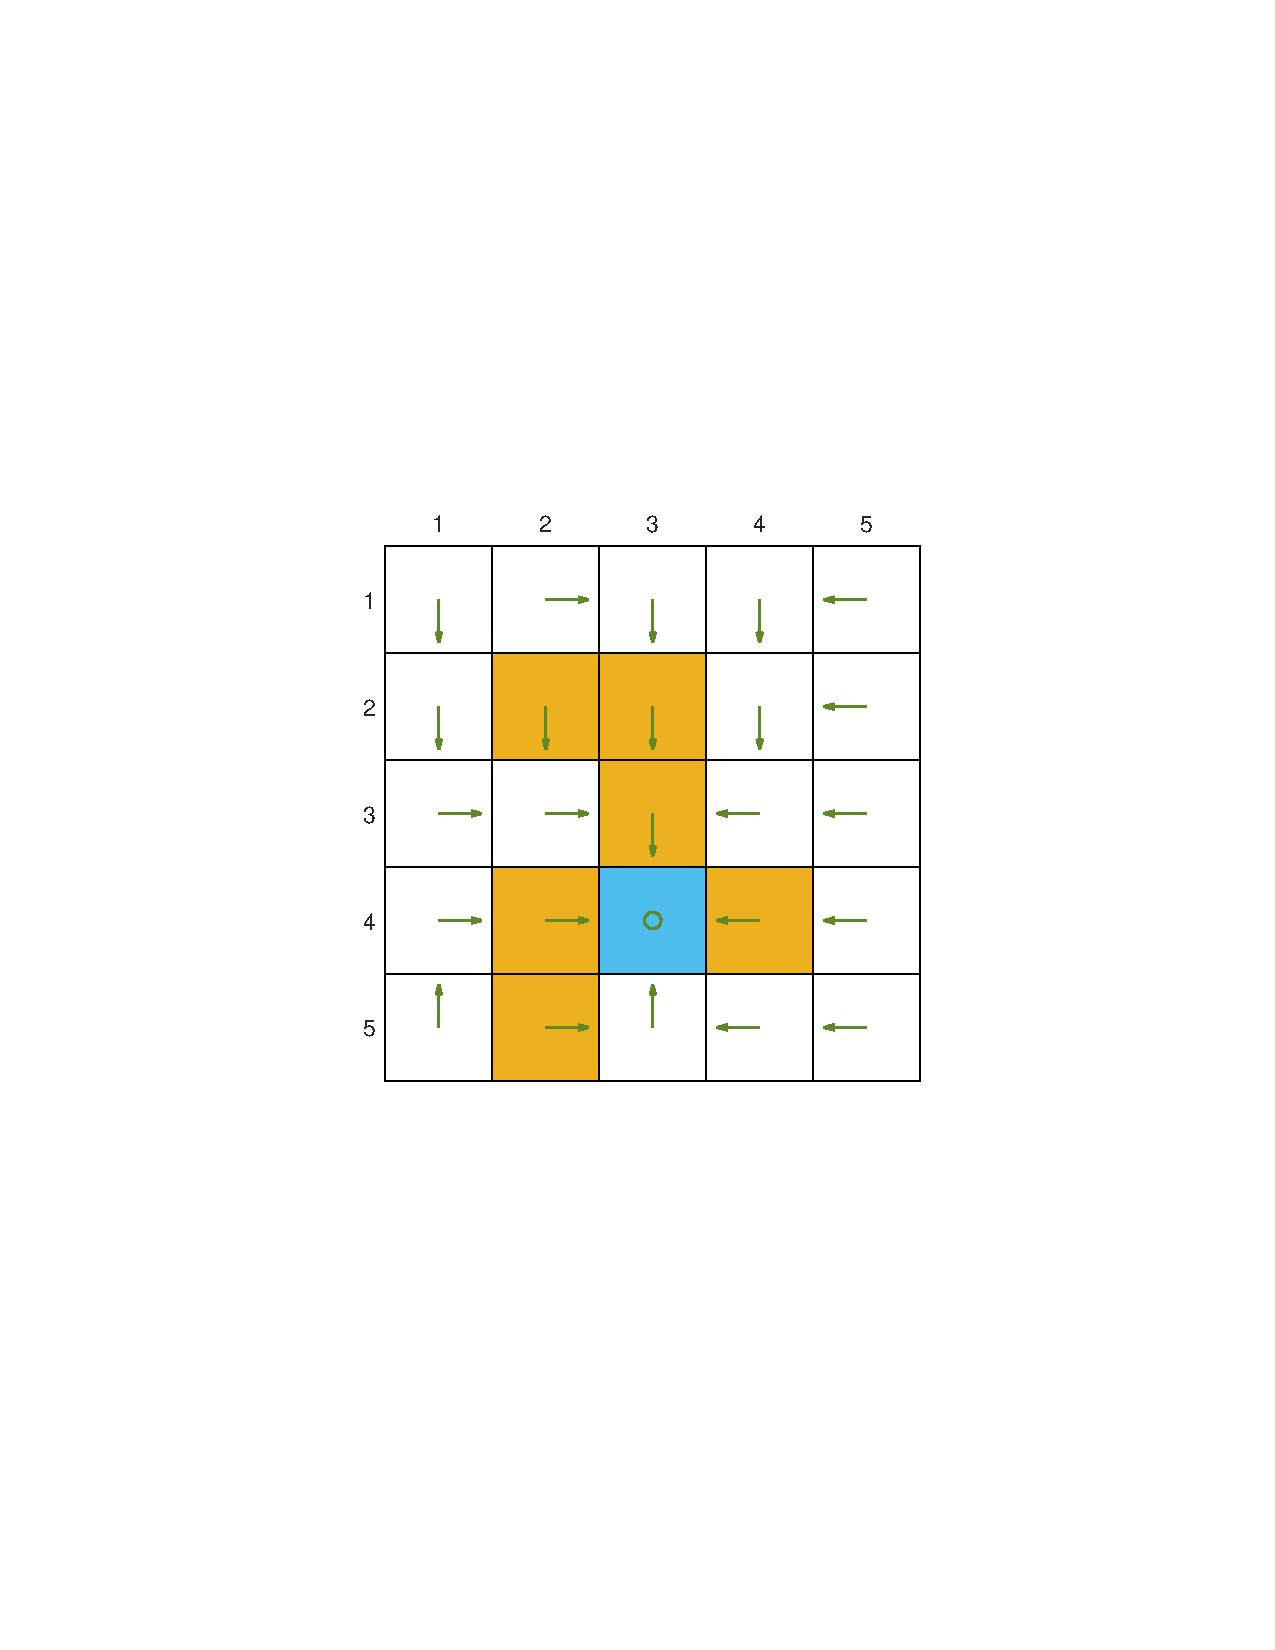
\includegraphics[width=0.25\linewidth]{figures_offpolicy/fig_offPolicy_estimatedPolicy.pdf}\quad}
  \subfloat[State value error]{\quad\includegraphics[width=0.3\linewidth]{figures_offpolicy/fig_offPolicy_valueError.pdf}\quad}
\end{figure}
}
\end{frame}
%---------------------
\begin{frame}
\frametitle{Q-learning -- Examples}

The importance of exploration: episodes of $10^5$ steps

If the policy is not sufficiently exploratory, the samples are not good.
\begin{figure}[]
\setcounter{subfigure}{0}
  \centering
  \subfloat[Behavior policy $\epsilon=0.5$]{
  \includegraphics[width=0.3\linewidth]{figures_offpolicy/fig_offPolicy_behaviorPolicy_nonexploratory_epsi05.pdf}}\,
  \subfloat[Generated episode]{
  \includegraphics[width=0.3\linewidth]{figures_offpolicy/fig_offPolicy_episode_nonexploratory_epsi05.pdf}}\,
  \subfloat[Q-learning result]{
  \includegraphics[width=0.33\linewidth]{figures_offpolicy/fig_offPolicy_valueError_nonexploratory_epsi05.pdf}}
\end{figure}

\end{frame}
%---------------------
\begin{frame}
\frametitle{Q-learning -- Examples}
\vspace{-10pt}
\begin{figure}[]
\setcounter{subfigure}{0}
  \centering
  \subfloat[Behavior policy $\epsilon=0.1$]{
  \includegraphics[width=0.25\linewidth]{figures_offpolicy/fig_offPolicy_behaviorPolicy_nonexploratory_epsi01.pdf}}\, \subfloat[Generated episode]{
  \includegraphics[width=0.25\linewidth]{figures_offpolicy/fig_offPolicy_episode_nonexploratory_epsi01.pdf}}\,
  \subfloat[Q-learning result]{
  \includegraphics[width=0.3\linewidth]{figures_offpolicy/fig_offPolicy_valueError_nonexploratory_epsi01.pdf}}\\
  \setcounter{subfigure}{0}
  \subfloat[Behavior policy $\epsilon=0.1$]{
  \includegraphics[width=0.25\linewidth]{figures_offpolicy/fig_offPolicy_behaviorPolicy_nonexploratory_epsi01_rand.pdf}}\,
  \subfloat[Generated episode]{
  \includegraphics[width=0.25\linewidth]{figures_offpolicy/fig_offPolicy_episode_nonexploratory_epsi01_rand.pdf}}\,
  \subfloat[Q-learning result]{
  \includegraphics[width=0.3\linewidth]{figures_offpolicy/fig_offPolicy_valueError_nonexploratory_epsi01_rand.pdf}}
\end{figure}

\end{frame}
%--------------------------------------
\AtBeginSection[]% put it to the start of each section
{
  \begin{frame}
    \frametitle{Outline}
    \tableofcontents[currentsection]
  \end{frame}
}
\section{A unified point of view}
%---------------------
\begin{frame}
\frametitle{A unified point of view}

All the algorithms we introduced in this lecture can be expressed in a unified expression:
\red{
\begin{align*}%\label{chapterTD_eq_uniformTDAlgo}
q_{t+1}(s_t,a_t)
&=q_t(s_t,a_t)-\alpha_t(s_t,a_t)[q_t(s_t,a_t)-\blue{\bar{q}_t}]
\end{align*}}
where $\bar{q}_t$ is the \emph{TD target}.

\vspace{10pt}
\pause
Different TD algorithms have different $\bar{q}_t$.

\vspace{10pt}
\begin{tabular}{|p{3cm}||p{7cm}|}%{|p{0.45\textwidth}|p{0.45\textwidth}|}
  % after \\: \hline or \cline{col1-col2} \cline{col3-col4} ...
  \hline
  \textbf{Algorithm} & \textbf{Expression of $\bar{q}_t$} \\
  \hline
  Sarsa & \blue{$\bar{q}_t=r_{t+1}+\gamma q_t(s_{t+1},a_{t+1})$} \\
  \hline
$n$-step Sarsa & \blue{$\bar{q}_t=r_{t+1}+\gamma r_{t+2}+\dots+\gamma^n q_t(s_{t+n},a_{t+n})$} \\
  %\hline
  %  Expected Sarsa & \blue{$\bar{q}_t=r_{t+1}+\gamma\sum_a \pi_t(a|s_{t+1})q_t(s_{t+1},a)$} \\
  \hline
    Q-learning & \blue{$\bar{q}_t=r_{t+1}+\gamma\max_{a}q_t(s_{t+1},a)$} \\
  \hline
  Monte Carlo & \blue{$\bar{q}_t=r_{t+1}+\gamma r_{t+2}+\dots$} \\
  \hline
\end{tabular}

\vspace{10pt}
\pause
Remark: The MC method can also be expressed in this unified expression by setting $\alpha_t(s_t,a_t)=1$. In particular, the expression is $q_{t+1}(s_t,a_t)=\bar{q}_t$.

\end{frame}
%---------------------
\begin{frame}
\frametitle{A unified point of view}

All the TD algorithms can be viewed as stochastic approximation algorithms solving the Bellman equation or Bellman optimality equation:

\vspace{15pt}
{\footnotesize
\begin{tabular}{|p{1.5cm}||p{8.7cm}|}%{|p{0.45\textwidth}|p{0.45\textwidth}|}
  % after \\: \hline or \cline{col1-col2} \cline{col3-col4} ...
  \hline
  \textbf{Algorithm} & \textbf{Equation to solve }\\
  \hline
  Sarsa & \blue{BE:
$q_\pi(s,a)=\E\left[R_{t+1}+\gamma q_\pi(S_{t+1},A_{t+1})|S_t=s,A_t=a\right]$} \\
  \hline
$n$-step Sarsa & \blue{BE: $q_\pi(s,a)=\E[R_{t+1}+\gamma R_{t+2}+\dots+\gamma^n q_\pi(s_{t+n},a_{t+n})|S_t=s,A_t=a]$} \\
  %\hline
  %  Expected Sarsa & \blue{BE: $q_\pi(s,a)=\E\big[R_{t+1}+\gamma \E_{A_{t+1}}[q_\pi(S_{t+1},A_{t+1})]\big|S_t=s,A_t=a\big]$} \\
  \hline
    Q-learning & \red{BOE: $q(s,a)=\E\left[R_{t+1}+\gamma\max_{a}q(S_{t+1},a)\big|S_t=s,A_t=a\right]$} \\
  \hline
  Monte Carlo & \blue{BE: $q_\pi(s,a)=\E[R_{t+1}+\gamma R_{t+2}+\dots|S_t=s,A_t=a]$} \\
  \hline
\end{tabular}
}
\end{frame}
%--------------------------------------
\AtBeginSection[]% put it to the start of each section
{
  \begin{frame}
    \frametitle{Outline}
    \tableofcontents[currentsection]
  \end{frame}
}
\section{Summary}
%---------------------
\begin{frame}
\frametitle{Summary}

\begin{itemize}
\item Introduced various TD learning algorithms

\item Their expressions, math interpretations, implementation, relationship, examples

\item Unified point of view
\end{itemize}

\end{frame}
%---------------------
%%%%%%%%%%%%%%%%%%%%%%%%%%%%%%%%%%%%%%%%%%%%%%%%%%%%%%%%%%%%%%%%%%%%%%%%%%%%%%%%%%%%%%%%%%%%%%%%%%
%\bibliographystyle{plainnat}
%\bibliography{myOwnPub,zsyReferenceAll}
\end{document}
